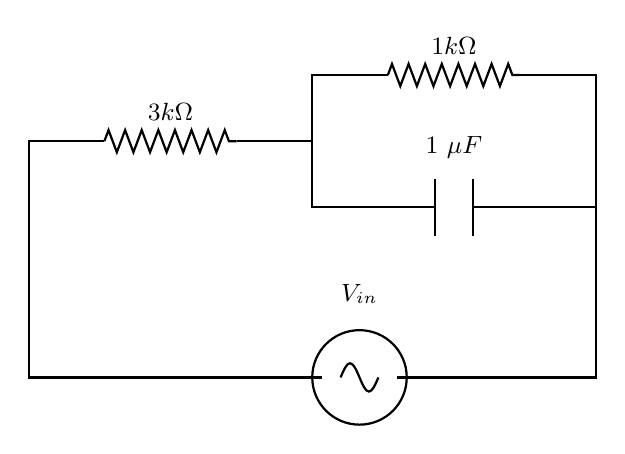
\begin{tikzpicture}[scale=1.2, every node/.style={font=\small}]

  % Top left wire & 3 k\Omega resistor
  \draw[thick] (0,-1) -- (0,1.5) -- (0.8,1.5);
  \draw[thick, decorate, decoration={zigzag, segment length=6pt, amplitude=4pt}] (0.8,1.5) -- (2.2,1.5);
  \node[above=4pt] at (1.5,1.5) {$3\text{ k}\Omega$};
  \draw[thick] (2.2,1.5) -- (3,1.5);
  
  % Parallel top branch: 1 k\Omega resistor
  \draw[thick] (3,1.5) -- (3,2.2) -- (3.8,2.2);
  \draw[thick, decorate, decoration={zigzag, segment length=6pt, amplitude=4pt}] (3.8,2.2) -- (5.2,2.2);
  \node[above=4pt] at (4.5,2.2) {$1\text{ k}\Omega$};
  \draw[thick] (5.2,2.2) -- (6,2.2) -- (6,1.5);
  
  % Parallel bottom branch: 1 \mu F capacitor
  \draw[thick] (3,1.5) -- (3,0.8) -- (4.3,0.8);
  \draw[thick] (4.3,0.5) -- (4.3,1.1);
  \draw[thick] (4.7,0.5) -- (4.7,1.1);
  \node[above=4pt] at (4.5,1.1) {$1\ \mu\text{F}$};
  \draw[thick] (4.7,0.8) -- (6,0.8);
  
  % Outer connections & AC Source
  \draw[thick] (6,1.5) -- (6,-1) -- (3.9,-1);
  \draw[thick] (0,0) -- (0,-1) -- (3.1,-1);
  \draw[thick] (3.5,-1) circle (0.5);
  \draw[thick] (3.3,-1) sin (3.4,-0.85) cos (3.5,-1) sin (3.6,-1.15) cos (3.7,-1);
  \node[above=6pt] at (3.5,-0.5) {$V_{\text{in}}$};
\end{tikzpicture}

